% G-CEZO PA-28-161 Cadet -- operating checklist
% PART A: Redhill & Shoreham Aviation "Piper PA28 Checklist", 31st March 2021 - Revision 1.0
%         ("PA28 2021 Checklist DRAFT v2.pdf"), reproduced word for word, including its own item
%         numbering (some numbers are skipped or repeated in the original) and spelling.
%         Grey "POH" notes are references to the G-CEZO POH (Report VB-1360) only; they are
%         not checklist items. Notes marked "differs" show where the POH figure is different.
% LAYOUT: Pooleys-style flip-over checklist (A5, top binding margin, item .... action rows,
%         coloured running header: black normal, red emergencies, grey reference, blue POH).
% PART B: the POH checklists and emergency procedures, verbatim (poh-body.tex).
% Do not edit checklist wording without explicit approval -- see CLAUDE.md.
\documentclass[10pt]{article}
% Shared LaTeX style for the G-CEZO checklists (formatting only, no checklist content).
\usepackage[utf8]{inputenc}
\usepackage[T1]{fontenc}
\usepackage{helvet}
\renewcommand{\familydefault}{\sfdefault}
\usepackage[a5paper,margin=10mm,top=14mm,bottom=14mm]{geometry}
\usepackage{fancyhdr}
\usepackage{zref-totpages}
\usepackage{xcolor}
\usepackage{titlesec}
\usepackage{enumitem}
\usepackage{needspace}
\usepackage{multicol}
\usepackage{textcomp}

\definecolor{emerg}{RGB}{170,0,0}
\definecolor{normal}{RGB}{0,70,140}

\pagestyle{fancy}
\fancyhf{}
\fancyhead[L]{\small G-CEZO \textbullet\ PA-28-161 Cadet}
\fancyhead[R]{\small\nouppercase{\leftmark}}
\fancyfoot[C]{\small Page \thepage\ of \ztotpages}
\fancyfoot[R]{\scriptsize Source: POH VB-1360}
\fancyfoot[L]{\scriptsize\bfseries\color{red}UNOFFICIAL \textendash\ FOR REFERENCE ONLY}
\renewcommand{\headrulewidth}{0.4pt}

\setlength{\parindent}{0pt}
\setlength{\parskip}{2pt}

\titleformat{\section}{\Large\bfseries}{}{0pt}{}[\titlerule]
\titleformat{\subsection}{\normalsize\bfseries}{}{0pt}{}
\titleformat{\subsubsection}{\small\bfseries\itshape}{}{0pt}{}
\titlespacing*{\subsection}{0pt}{8pt}{3pt}
\titlespacing*{\subsubsection}{0pt}{5pt}{2pt}

% \chk{Item}{ACTION} -- item ............ ACTION
\newcommand{\chk}[2]{\par{\noindent\parfillskip=0pt\hangindent=2em #1\ \dotfill\ #2\par}}
% Plain line (instruction text, no action column)
\newcommand{\txt}[1]{\par\noindent #1\par}
% Condition / lead-in line
\newcommand{\cond}[1]{\par\vspace{3pt}\noindent #1\par}
% Boxed NOTE / CAUTION / WARNING exactly as printed
\newcommand{\pohnote}[2]{\par\vspace{3pt}\begin{center}\begin{minipage}{0.82\linewidth}\centering\textbf{#1}\\[1pt]\small\raggedright #2\end{minipage}\end{center}\vspace{2pt}}

\newenvironment{proc}[1]{\needspace{6\baselineskip}\subsection*{#1}\begin{list}{}{\leftmargin=1em\rightmargin=0pt\itemsep=0pt\parsep=0pt\topsep=0pt}\item\relax}{\end{list}}


\usepackage{graphicx}
\usepackage{tabularx}
\usepackage{colortbl}
\geometry{a5paper,left=9mm,right=9mm,top=24mm,bottom=12mm,headsep=5mm,headheight=14pt}
\newcommand{\barcol}{black}\newcommand{\bartext}{NORMAL}
\fancyhf{}\renewcommand{\headrulewidth}{0pt}
\fancyhead[C]{{\setlength{\fboxsep}{2.5pt}\colorbox{\barcol}{\parbox{\dimexpr\textwidth-5pt}{\color{white}\footnotesize\bfseries G-CEZO \textbullet\ PA-28-161 \hfill \bartext}}}}
\fancyfoot[C]{\footnotesize \thepage}
\fancyfoot[R]{}
\fancyfoot[L]{\scriptsize\bfseries\color{red}UNOFFICIAL \textendash\ FOR REFERENCE ONLY}

\definecolor{rhgray}{RGB}{230,231,232}
\definecolor{rhbar}{RGB}{128,129,132}
\definecolor{empink}{RGB}{251,215,215}
\definecolor{emred}{RGB}{211,35,42}
\definecolor{pohc}{RGB}{40,90,140}
\definecolor{pohdiff}{RGB}{170,90,0}

\newcounter{rhrow}
% Section bar (black), sub-section bar (grey), emergency title (red frame, pink fill)
\newcommand{\rhsec}[1]{\par\needspace{9\baselineskip}\vspace{7pt}\noindent{\setlength{\fboxsep}{3pt}\colorbox{black}{\parbox{\dimexpr\linewidth-6pt}{\color{white}\bfseries #1}}}\par\vspace{2pt}\setcounter{rhrow}{0}\addcontentsline{toc}{subsection}{#1}}
\newcommand{\rhsub}[1]{\par\needspace{6\baselineskip}\vspace{2pt}\noindent{\setlength{\fboxsep}{3pt}\colorbox{rhbar}{\parbox{\dimexpr\linewidth-6pt}{\centering\color{white}\bfseries #1}}}\par\vspace{2pt}\setcounter{rhrow}{0}}
\newcommand{\emsec}[1]{\par\needspace{5\baselineskip}\vspace{7pt}\noindent{\setlength{\fboxsep}{3pt}\setlength{\fboxrule}{1.2pt}\fcolorbox{emred}{empink}{\parbox{\dimexpr\linewidth-8.4pt}{\bfseries #1}}}\par\vspace{2pt}\setcounter{rhrow}{0}\addcontentsline{toc}{subsection}{#1}}
% Numbered row: \rh{number}{item}{action}  (alternate rows shaded, as in the original)
\newcommand{\rhbg}{white}
\newcommand{\rhOLD}[3]{\stepcounter{rhrow}\ifodd\value{rhrow}\renewcommand{\rhbg}{white}\else\renewcommand{\rhbg}{rhgray}\fi
  \par\noindent{\setlength{\fboxsep}{2pt}\colorbox{\rhbg}{\parbox[t]{\dimexpr\linewidth-4pt}{\small\makebox[1.8em][l]{#1}\parbox[t]{0.36\linewidth}{\raggedright #2\strut}\hspace{4pt}\parbox[t]{\dimexpr0.64\linewidth-1.8em-10pt}{\raggedright #3\strut}}}}\par\vspace{-\parskip}}
% Full-width numbered row: \rhw{number}{text}
\newcommand{\rhwOLD}[2]{\stepcounter{rhrow}\ifodd\value{rhrow}\renewcommand{\rhbg}{white}\else\renewcommand{\rhbg}{rhgray}\fi
  \par\noindent{\setlength{\fboxsep}{2pt}\colorbox{\rhbg}{\parbox[t]{\dimexpr\linewidth-4pt}{\small\makebox[1.8em][l]{#1}\parbox[t]{\dimexpr\linewidth-1.8em-6pt}{\raggedright #2\strut}}}}\par\vspace{-\parskip}}
\newcommand{\rh}[3]{{\small\par\noindent\parfillskip=0pt\hangindent=1.9em\hangafter=1 \makebox[1.9em][l]{#1}#2\ \dotfill\ #3\par}\vspace{1.2pt}}
\newcommand{\rhw}[2]{{\small\par\noindent\hangindent=1.9em\hangafter=1 \makebox[1.9em][l]{#1}#2\par}\vspace{1.2pt}}
% Dotted-leader item (walk-round pages)
\newcommand{\dl}[2]{\par{\small\noindent\parfillskip=0pt #1\ \dotfill\ #2\par}}
% POH reference note (not a checklist item)
\newcommand{\pohref}[1]{\par\vspace{1pt}\noindent{\scriptsize\color{pohc}\setlength{\fboxsep}{1pt}\fcolorbox{pohc}{white}{\textbf{POH}}\ \itshape #1}\par\vspace{1pt}}
\newcommand{\pohdif}[1]{\par\vspace{1pt}\noindent{\scriptsize\color{pohdiff}\setlength{\fboxsep}{1pt}\fcolorbox{pohdiff}{white}{\textbf{POH differs}}\ \itshape #1}\par\vspace{1pt}}
\newcommand{\cnp}{\par\hfill{\small\itshape Continues on next page}\par}

\begin{document}
\setlength{\headwidth}{\textwidth}
\thispagestyle{empty}
\begin{center}
\vspace*{14mm}
{\huge\bfseries Redhill \& Shoreham\\[4pt] Aviation}\\[16mm]
{\LARGE\bfseries Piper PA28}\\[6pt]
{\Large Checklist}\\[10mm]
{\Large\bfseries\color{red} UNOFFICIAL \textendash\ FOR REFERENCE ONLY}\\[6mm]
{\normalsize\bfseries G-CEZO edition (PA-28-161 Cadet)}\\[2pt]
{\footnotesize with references to the G-CEZO POH (Report VB-1360)}\\[14mm]
\end{center}
Name: \rule{0.7\linewidth}{0.4pt}\\[8mm]
\begin{center}{\small\color{gray}31\textsuperscript{st} March 2021 - Revision 1.0}\end{center}
\vfill
\noindent\fcolorbox{emred}{empink}{\parbox{\dimexpr\linewidth-2\fboxsep-2\fboxrule}{\scriptsize\textbf{FOR REFERENCE AND DOUBLE-CHECKING ONLY.}
Unofficial transcription. Part A is the Redhill \& Shoreham checklist as printed; boxed \textbf{POH} notes are references to the
G-CEZO POH and are not checklist items; Part B reproduces the POH checklists. The POH/AFM and the operator's procedures are authoritative.
The pilot in command is responsible for the flight. Provided ``as is'' without warranty; to the fullest extent permitted by law no liability
is accepted for any loss, damage, injury or death arising from its use.}}

\clearpage
\tableofcontents

%=====================================================================
\clearpage
\section*{Part A --- Normal Checklist (Redhill \& Shoreham, Rev 1.0)}
\addcontentsline{toc}{section}{Part A --- Normal Checklist (Redhill \& Shoreham)}
\markboth{Part A --- Normal}{}

\rhsec{External Checks}
{\small Check documents are current and correct. Visually check the aircraft's general condition.
Remove tie-down ropes, pitot head cover, chocks and any external control locks. In cold
weather, remove even small accumulations of frost, ice or snow from the aircraft.\par\smallskip
Check that the aircraft is parked in a free area, so that it may easily move onto the taxyway.
Check that a fire extinguisher is available.\par}
\begin{center}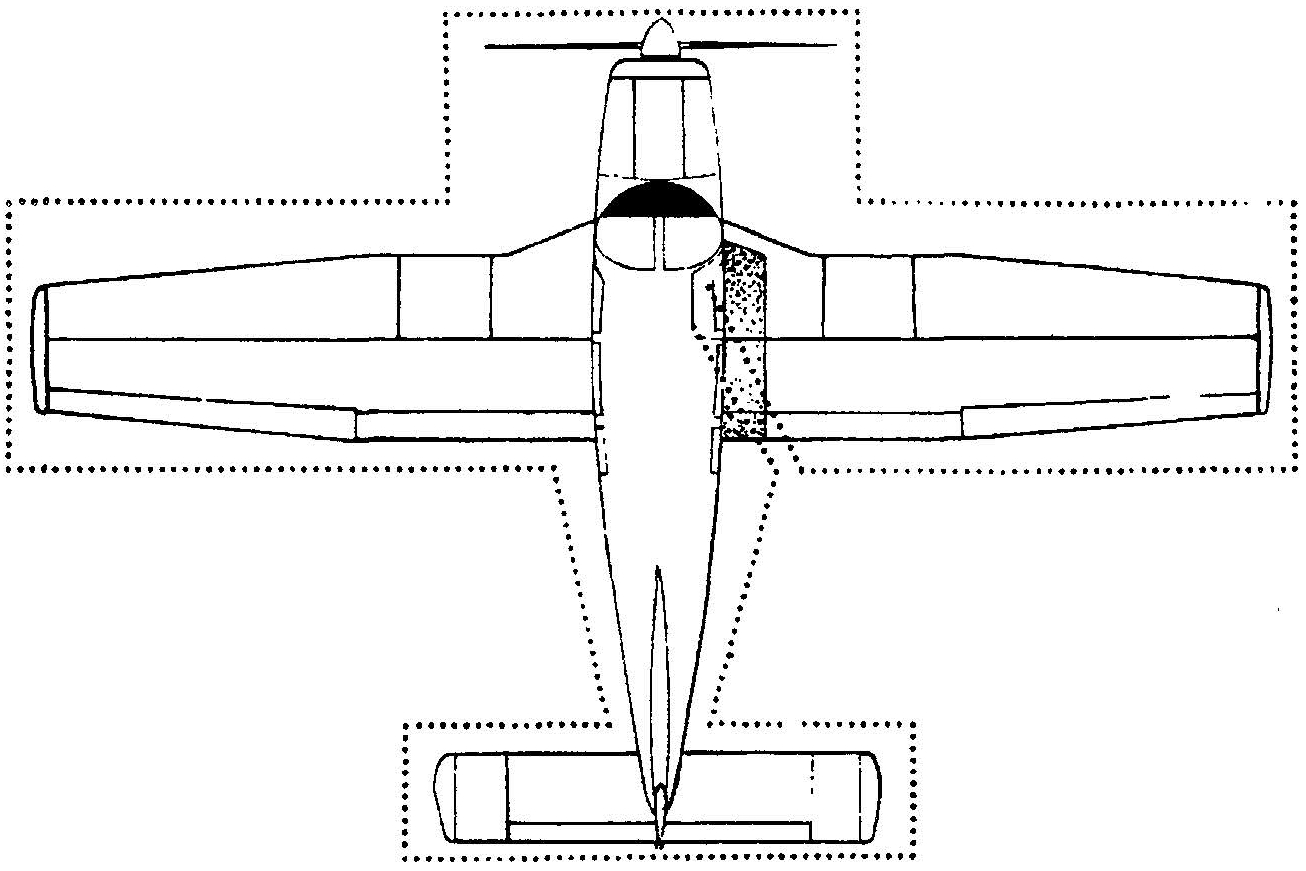
\includegraphics[width=0.62\linewidth]{checklist-assets/rh_p2_x4.png}\end{center}
\pohref{4.5a Preparation (4.9) and 4.5b Preflight Checklists (4.11) --- see Part B.}

\subsection*{1. Cockpit Preparation}
\dl{Aircraft Documents}{Stowed}
\dl{Parking Brake}{On}
\dl{I.F. Screens}{Stowed}
\dl{First Aid Kit}{Stowed}
\dl{Fire Extinguisher}{Checked}
\dl{Magneto Switches}{Off}
\dl{Avionics Master Switch}{Off}
\dl{Circuit Breakers}{Check In}
\dl{Trim Indicator}{Correct Movement/Set}
\dl{Flying Controls}{Full Free Correct Movement}
\dl{Battery Switch}{On}
\dl{Pitot Heat}{On}
\dl{Fuel Contents}{Check}
\dl{Fuel selector}{Emptier Tank}
\dl{Annunciator/low voltage lights}{Test/On}
\begin{center}\small *Leave cockpit and check externally as necessary, and then re-enter cockpit before\\ carrying out full external pre-flight inspection.\end{center}
\dl{*Recognition/landing lights}{On/Check/Off}

\subsection*{1. Cockpit Preparation (Continued)}
\dl{*Anti-collision lights}{On/Check/Off}
\dl{*Navigation lights}{On/Check/Off (Leave on at night)}
\dl{*Pitot heater}{On/Check/Off}
\dl{*Stall Warner}{On/Check/Off}
\dl{*Panel lighting}{Check (Leave on at night)}
\dl{Battery switch}{Off}
\dl{Pitot static drains}{Operate}
\dl{Flaps}{Fully Down/Check All Stages}
\pohref{4.11a COCKPIT --- see Part B. It also includes: Mixture \dots\ IDLE CUT-OFF; Trim \dots\ CHECK, SET NEUTRAL.}

\subsection*{2. External: Cabin Upper Fuselage}
\dl{Door}{Closed Flush}
\dl{Starboard Windows}{Clean}
\dl{Upper Fuselage}{Check/Undamaged}
\dl{Towbar (If Carried)}{Stowed}
\dl{Baggage Door}{Secure}

\subsection*{3. Starboard Wing}
\dl{Flap}{Check/Undamaged}
\dl{Aileron (Surface, Hinges \& Static Wicks)}{Check/ Undamaged}
\dl{Wing Tip}{Undamaged}
\dl{Strobe \& Navigation Light}{Undamaged}
\dl{Wing Surfaces}{Undamaged}
\dl{Fuel Tank (Contents, Cap Secure, Vent, Drain, No Seepage)}{Check}
\dl{Main Gear (Oleo Extension 4\textonehalf'')}{Check Security}
\dl{Tyre (Inflation, Creep, No Damage)}{Check}
\dl{Brakes (Pads, No Hydraulic Leaks, Undamaged)}{Check}
\dl{Fresh Air Intake}{Unobstructed}
\pohref{4.11b RIGHT WING: Main Gear Strut \dots\ PROPER INFLATION (4.50 in.)}

\subsection*{4. Nose Section}
\dl{Windscreen}{Clean}
\dl{OAT Probe}{Check}
\dl{Oil Contents (8 Qts Min 2 Qts, Recommended Minimum 6 Qts)}{Check/Cap Secure}
\dl{Starboard Cowling}{Secure}
\dl{Propeller/Spinner}{Undamaged/Secure}
\dl{Air Intakes}{Unobstructed}
\dl{Alternator Belt}{Check Tension}
\cnp

\subsection*{4. Nose Section (Continued)}
\dl{Landing Light}{Undamaged}
\dl{Nose Gear (Oleo Extension 3\textonequarter'')}{Check Security}
\dl{Tyre (Inflation, Creep, No Damage)}{Check}
\dl{Brake Fluid}{Check}
\dl{Port Cowling}{Secure}
\dl{Fuel Drain}{Sample/No Seepage}
\dl{Port Window}{Clean}
\pohref{4.11c NOSE SECTION: Nose Gear Strut \dots\ PROPER INFLATION (3.25 in.); Fuel Strainer \dots\ DRAIN, CHECK for water, sediment and proper fuel.}

\subsection*{5. Port Wing}
\dl{Fresh Air Intake}{Unobstructed}
\dl{Brakes (Pads, No Hydraulic Leaks, Undamaged)}{Check}
\dl{Tyre (Inflation, Creep, No Damage)}{Check}
\dl{Main Gear (Oleo Extension 4\textonehalf'')}{Check Security}
\dl{Fuel Tank (Contents, Cap Secure, Vent, Drain, No Seepage)}{Check}
\dl{Pitot Head/Static}{Unobstructed/Secure}
\dl{Stall Warning Vane}{Free/Undamaged}
\dl{Wing Surfaces}{Undamaged}
\dl{Wing Tip}{Undamaged}
\dl{Strobe \& Navigation Light}{Undamaged}
\dl{Aileron (Surface, Hinges \& Static Wicks)}{Check/ Undamaged}
\dl{Flap}{Check/Undamaged}
\pohref{4.11d LEFT WING: Main Gear Strut \dots\ PROPER INFLATION (4.50 in.); Pitot/Static Head \dots\ REMOVE COVER - HOLES CLEAR.}

\subsection*{6. Rear Fuselage, Fin And Stabilator}
\dl{Radio Aerials}{Secure}
\dl{Port Fuselage \& Window}{Undamaged/Clean}
\dl{Fresh Air Intake}{Check}
\dl{Fin Surface}{Undamaged/Secure}
\dl{Rudder \& Nav Light}{Undamaged}
\dl{Stabilator}{Free/Undamaged}
\dl{Air Conditioning Scoop (If Fitted)}{Flush/Undamaged}
\dl{Starboard Fuselage \& Window}{Undamaged/Clean}
\dl{Static Vents (If Fitted)}{Unobstructed/Clean}
\pohref{4.11e FUSELAGE --- see Part B.}

\clearpage
\rhsec{Before Engine Start Checks}
\rh{1.}{Flaps}{Retracted}
\rh{2.}{External Checks}{Completed}
\rh{3.}{Passenger Briefing}{Completed}
\rh{4.}{Cabin Door}{Closed \& Latched}
\rh{5.}{Seats\\Seat Backs Upright}{Adjusted \& Locked}
\rh{6.}{Seat Belts \& Shoulder Straps}{Fitted \& Secure}
\rh{7.}{Alternate Static Selector (If Fitted)}{Check/Normal}
\rh{8.}{Flight Instruments\\Standby Compass \& Deviation Card}{Check Condition}
\rh{9.}{Battery Master Switch}{On}
\rh{10.}{Annunciator/Low Voltage Light}{Check/On}
\rh{11.}{VAC Off Caption}{On}
\rh{12.}{Avionics/Radio Master Switch}{Off}
\pohref{4.5c Before Starting Engine (4.13): Brakes \dots\ SET; Carburetor Heat \dots\ FULL OFF; Fuel Selector \dots\ DESIRED TANK; Avionics \dots\ OFF; ALTR Switch \dots\ ON.}

\rhsec{Starting}
\rh{1.}{Anti-Collision Light}{On}
\rh{2.}{Fuel Selector}{Tank With Lowest Contents}
\rh{3.}{Mixture}{Exercise/Set Rich}
\rh{4.}{Throttle}{Exercise/Set \textonequarter''}
\rh{5.}{Electric Fuel Pump}{On, check pressure, Off}
\rh{6.}{Prime}{As Required \& Lock}
\rh{7.}{Lookout}{Clear All Round, Open Window ``CLEAR PROP''}
\rh{8.}{Magnetos}{On Both}
\rh{9.}{Starter}{Operate \& Release as Soon as Engine Starts}
\pohref{4.5d Engine Start (4.15). Cold engine: Throttle \dots\ \textonequarter\ INCH OPEN; ``If engine does not start within 10 sec., prime and repeat starting procedure.'' Hot engine: Throttle \dots\ \textonehalf\ INCH OPEN. Flooded: Throttle OPEN FULL, Electric Fuel Pump OFF, Mixture IDLE CUT-OFF --- see Part B.}

\rhsec{After Start}
\rh{1.}{Starter Warning Light}{Out, If Not Immediately Turn Magnetos Off}
\rh{2.}{Oil Pressure}{Within 30 secs 25 PSI Minimum (If Not, Shut down)}
\rh{3.}{RPM}{Set to 1200}
\rh{4.}{Alternator/Ammeter}{On \& Holding Positive Charge}
\rh{6.}{Low Voltage Light}{Out}
\rh{7.}{Suction}{Check Registering, VAC off Caption Out}
\rh{8.}{Annunciator Panel Lights}{All Out}
\rh{9.}{Fuel Pressure}{Check}
\rh{10.}{Avionics/Radio Master Switch}{On (If Fitted)}
\rh{11.}{Electric Trim (If Fitted)}{Check}
\rh{12.}{Flight Instruments}{Check (AI erect, DI set, VSI, Turn Co-ord flag away) HSI/RMI Heading, Standby Compass/Slaving Meter}
\rh{13.}{Avionics}{Checked and Set As Required}
\rh{14.}{Auto-Pilot (If Fitted)}{Check and Off}
\rh{15.}{Magnetos}{Check at 1200 RPM}
\rh{16.}{Radios}{Radio Check, ATIS (if available) \& Taxi Clearance}
\rh{17.}{Altimeters}{Cross Check \& Set}
\pohref{2.7(e) Oil Pressure Minimum (red line) 25 PSI. 4.17 Engine Warm-Up: Throttle \dots\ 800 to 1200 RPM.}

\rhsec{Taxying}
\rh{1.}{Brakes \& Nosewheel Steering}{Check Operation Satisfactory For Both Pilots}
\rh{2.}{Flight Intruments}{During Turns Check Compass \& D.I turning in same direction, turn Indicator: Turn \& Skid. AI steady}
\pohref{4.5f Taxiing (4.19) --- see Part B.}

\clearpage
\rhsec{Power Checks}
\rh{1.}{Position}{Into wind. Avoid Rough Ground and Loose Stones. Clear of Aircraft and Personnel}
\rh{2.}{Parking Brake}{On}
\rh{3.}{Fuel Selector}{Change Tank to Fuller Tank}
\rh{4.}{RPM}{Check Clear All Round. Set to 2000}
\rh{5.}{Carb. Heat}{Check Operation \& Return to Cold}
\rh{6.}{Magnetos}{Check Each Magneto in Turn. Max Permissible Drop 175 RPM; and Max. Differential is 50 RPM}
\rh{7.}{Alternator Output}{Check}
\rh{8.}{Suction}{4.9 to 5.1'' Hg.}
\rh{9.}{Temperature \& Pressure}{Check, Steady and Within Limits}
\rh{10.}{RPM}{Smoothly Close the Throttle, Check Idle.Temps and Pressures Steady, Within Limits. Then Reset 1200}
\pohref{4.21 Ground Check: Throttle \dots\ 2000 RPM; Magnetos \dots\ max. drop 175 RPM -max. diff. 50 RPM.}
\pohdif{4.21 Ground Check: Vacuum \dots\ 4.8 to 5.1 in. Hg (Redhill item 8: 4.9 to 5.1'' Hg).}

\rhsec{Pre-Takeoff Checks}
\rh{1.}{Trim}{Set for Take-Off}
\rh{2.}{Throttle Friction}{Finger Tight}
\rh{3.}{Mixture}{Mixture Rich.}
\rh{4.}{Magnetos}{Magnetos on Both. Master Switch On}
\rh{5.}{Carb Heat}{Off}
\rh{6.}{Fuel Selector}{On Fuller Tank, Check Contents}
\rh{7.}{Fuel Pump}{On, Pressure Checked}
\rh{8.}{Flaps}{Set (Normal 0\textdegree)}
\rh{9.}{Engine Instruments}{Check (Temperatures \& Pressures)}
\rh{10.}{Seat Belts / Seat Backs}{Secure/Erect}
\rh{11.}{Cabin Doors}{Locked/Latched}
\rh{12.}{Annunciator Panel}{Test/All Lights Out}
\rh{13.}{Flying Controls}{Full Free Correct Movement}
\rh{15.}{Radio \& Transponder}{Confirm Radio/Nav Set. Transponder set, Alt.}
\rh{16.}{Flight Instruments}{Check/Altimeters Set. Pitot Heat as Required}
\rh{17.}{Lights}{Recognition/Landing Lights and Anit-Cols Lights On}
\rh{18.}{Take-Off Brief}{Review Speeds, Crosswind, Departure Brief \& Emergency Procedures}
\pohref{4.5h Before Takeoff (4.23) and the 2.23 TAKEOFF CHECKLIST placard --- see Part B.}

\rhsec{Take Off}
\rhsub{Normal Take-Off}
\rh{1.}{Lookout}{Obtain Clearance, Check Approach Clear Visually}
\rh{2.}{Line up}{On Runway Centreline, Ensure Nosewheel Straight, D.I. Indicating Runway Heading. Controls Free}
\rh{3.}{Brakes}{Off, Heels on Floor}
\rh{4.}{Throttle}{Smoothly Open to Full; Check Power}
\rh{5.}{Oil}{Temperature and Pressure Steady and in Green}
\rh{6.}{Airspeed}{Increasing}
\rh{7.}{Elevator Control}{Lift Nose by 60 Kts}
\rh{8.}{Climb Speed}{80 Kts (Clean).}
\pohref{4.25a Normal: Accelerate to 45 to 55 KIAS; Control Wheel \dots\ back pressure to rotate to climb attitude.}
\pohdif{4.3(a) Best Rate of Climb Speed 79 KIAS (Redhill item 8: 80 Kts).}
\rhsub{Short Field Take-Off (Hard Surface)}
\rh{1.}{Flaps}{25\textdegree}
\rh{2.}{Brakes}{Hold (Keep Moving During a Soft Field Take-Off)}
\rh{3.}{Throttle}{Fully Open, Check power, Oil Temp and Pressure}
\rh{4.}{Brakes}{Release}
\rh{5.}{Elevator Control}{Slight Back Pressure}
\rh{6.}{Climb Speed}{80 Kts (Best angle of Climb is 65 Kts)}
\pohref{4.25c 25\textdegree\ Flaps Takeoff: Accelerate to 40-50 KIAS (depending on weight) \dots\ maintain 44 to 55 KIAS (depending on weight) until obstacle clearance is achieved and climb out at 79 KIAS.}
\pohdif{4.3(b) Best Angle of Climb Speed 63 KIAS (Redhill item 6: 65 Kts); 4.3(a) Best Rate 79 KIAS (Redhill: 80 Kts).}

\rhsec{After Take-Off}
\rh{1.}{Lookout}{Point Selected Left of Nose, Check Drift}
\rh{2.}{Flaps}{Retract Above 200' a.g.l, Not Below 65 Kts}
\rh{3.}{Oil}{Temperature and Pressure Steady, Within Limits}
\rh{4.}{Recognition/Landing Lights}{Off}
\rh{5.}{Fuel Pump}{Off (Above 1000ft a.g.l)}
\pohref{4.25c Flaps \dots\ RETRACT SLOWLY. 4.27 Electric Fuel Pump \dots\ OFF at desired altitude.}

\rhsec{Climb}
\rhsub{Normal Climb}
\rh{1.}{Airspeed}{Clean: 80 Kts (Best Rate of Climb)}
\rh{2.}{Throttle}{Fully Open}
\rh{3.}{Mixture}{Rich Below 3000'}
\pohdif{4.27 Best Rate Climb Speed (Flaps Up) 79 KIAS (Redhill item 1: 80 Kts).}

\clearpage
\rhsub{En-Route Climb}
\rh{1.}{Airspeed}{90 Kts}
\rh{2.}{Throttle}{Fully Open}
\rh{3.}{Mixture}{As Required}
\pohdif{4.27 En Route 87 KIAS (Redhill item 1: 90 Kts).}

\rhsec{En-Route Checks (FREDA)}
\rh{1.}{\textbf{F}uel}{Check Contents/Balanced}
\rh{2.}{\textbf{R}adio / Radio aids}{Check Volume; Frequency Change if Required / Radio Aids Identified}
\rh{3.}{\textbf{E}ngine}{Oil Temperature and Pressure Steady and Within Limits. Ammeter Charging. Suction Within Limits. Check for Carb. Icing. Mixture as Required.}
\rh{4.}{\textbf{D}irection Indicator}{Check D.I.}
\rh{5.}{\textbf{A}ltimeter}{Set}
\pohref{4.5k Cruise (4.29): Normal Maximum Power \dots\ 75\%; Power \dots\ SET per power table; Mixture \dots\ ADJUST.}

\rhsec{HASELL Checks (Stalls)}
\rh{1.}{\textbf{H}eight}{Sufficient to Recover by 2000' AGL}
\rh{2.}{\textbf{A}irframe}{Flaps as Required. Brakes off}
\rh{3.}{\textbf{S}ecurity}{Doors, Windows and Harnesses Secure; No Loose Articles}
\rh{4.}{\textbf{E}ngine}{Check Oil Temperature and Pressure, Mixture as Required, Check Fuel Contents, Fuel Pump On, Clear Carb Ice}
\rh{5.}{\textbf{L}ocation}{Clear of Airfields, Built Up Areas, Controlled Airspace or Cloud and Danger Areas}
\rh{6.}{\textbf{L}ookout}{Check No Aircraft Around, Particularly Below}
\pohref{3.2a Stall speeds: 2325 lbs (0\textdegree\ Flap) 50 KIAS; 2325 lbs (Full Flap 44 KIAS. 3.3k Spin Recovery --- see Part B.}
\rhsub{HELL (For Continued Exercise)}
\rh{1.}{\textbf{H}eight}{Sufficient to Recover by 2000' AGL}
\rh{2.}{\textbf{E}ngine}{Check Oil Temperature and Pressure, Mixture as Required, Check Fuel Contents, Clear Carb Ice}
\rh{3.}{\textbf{L}ocation}{Clear of Airfields, Built Up Areas, Controlled Airspace or Cloud and Danger Areas}
\rh{4.}{\textbf{L}ookout}{Check No Aircraft Around, Particularly Below}
\par{\small\textbf{Note}: Reset D.I after completion of the exercise}\par

\rhsec{Airfield Approach Checks: FFREDA}
\rh{1.}{\textbf{F}uel}{Check Quantity/Balanced}
\rh{2.}{\textbf{F}uel Pump}{On}
\rh{2.}{\textbf{R}adio}{Correct Frequency Volume Up. Radio Aids Identified}
\rh{3.}{\textbf{E}ngine}{Temperature and Pressure in Limits, Mixture Rich}
\rh{4.}{\textbf{D}irection Indicator}{D.I. Reset}
\rh{5.}{\textbf{A}ltimeters}{Altimeters Set}

\rhsec{Pre-Landing Checks}
\rh{1.}{\textbf{B}rakes}{Brakes Off; Pressure Up}
\rh{2.}{\textbf{M}ixture}{Mixture Rich}
\rh{3.}{\textbf{C}arb. Heat}{Carb. Heat, Check for Icing and then Return to Cold}
\rh{4.}{\textbf{F}uel}{Fuel On, Sufficient for Go Around}
\rh{5.}{\textbf{O}il}{Oil Temperature and Pressure Within Limits}
\rh{6.}{\textbf{H}atches and Harnesses}{Pilot and Passenger Secure}
\rh{7.}{\textbf{L}ights}{Recognition/Landing Lights On}
\pohref{4.5n Approach and Landing (4.33) and the 2.23 LANDING CHECKLIST placard --- see Part B.}

\rhsec{Approach and Landing}
\rhsub{Normal Landing}
\rh{1.}{Carb. Heat}{Apply Full Heat Before Closing Throttle}
\rh{2.}{Flaps}{Select 25\textdegree\ When Speed is Below V\textsubscript{FE}}
\rh{3.}{Airspeed}{Initially 70 Kts. Final Approach, 63 Kts, Flap 40\textdegree}
\rh{4.}{Touchdown}{Mainwheels First, Lower Nose Wheel Gently}
\rh{5.}{Braking}{Minimum Required}
\pohref{4.33: Flaps \dots\ SET - 103 KIAS MAXIMUM; Trim to 70 KIAS; Final Approach Speed (Flaps 40\textdegree) \dots\ 63 KIAS. 2.5 White Arc (Flap Down) 44 KTS to 103 KTS.}
\rhsub{Flapless Landing}
\rh{1.}{Airspeed}{75 Kts}
\rhsub{Shortfield Landing}
\rh{1.}{Flaps}{40\textdegree}
\rh{2.}{Airspeed}{65 Kts}
\rh{3.}{Touchdown}{Main Wheels, Lower the Nose}
\rh{4.}{Brakes}{Apply Positively}
\pohdif{4.3(e) Landing Final Approach Speed (Flaps 40\textdegree) 63 KIAS (Redhill item 2: 65 Kts).}

\clearpage
\rhsec{Glide Approaches}
\rh{}{Airspeed}{75 Kts}
\rh{}{Flap}{As Required}
\par\smallskip{\small\noindent\textbf{Notes:}\quad 1.\ During prolonged glides; the engine should be warmed every 500'.\\
\hspace*{3.3em}2.\ The approach speeds are for calm conditions, in gusty or turbulent conditions the figures should be increased.}\par
\pohdif{3.2d Power Off Glide Speed 2325 lbs (0\textdegree\ Flap) 73 KIAS (Redhill: 75 Kts).}

\rhsec{Go-Around (Missed Approach)}
\rh{1.}{Throttle}{Full Power}
\rh{2.}{Carb. Heat}{Cold}
\rh{3.}{Airspeed}{65 Kts Until Clear of Obstacles, then 80 Kts}
\rh{4.}{Flaps}{If 30\textdegree, Retract to 25\textdegree\ as Soon as Possible. Retract Remaining 25\textdegree\ Above 200'}
\rh{5.}{Radio}{Inform ATC}
\pohref{4.3: Best Angle of Climb Speed 63 KIAS; Best Rate of Climb Speed 79 KIAS.}
\cnp

\rhsec{After Landing}
\begin{center}\small\bfseries Clear the runway and stop the aircraft\end{center}
\rh{1.}{Carb Heat}{Cold}
\rh{2.}{Flaps}{Up}
\rh{3.}{Fuel Pump}{Off}
\rh{3.}{Pitot heat}{Off}
\rh{4.}{Strobe Lights / Landing Lights}{Off / As Required}
\rh{5.}{Trimmers}{Set Neutral}
\rh{5.}{Transponder}{Standby}
\rh{6.}{Non-essential Electrics}{Off}

\rhsec{Shut Down}
\rh{1.}{Park}{Into Wind, Nosewheel Straight}
\rh{2.}{Parking brake}{On}
\rh{3.}{Engine}{1200 RPM for 30 secs; Check Oil Temperature and Pressure}
\rh{4.}{Magnetos}{Check}
\rh{5.}{Avionics/Radio Master Switch}{Off}
\rh{6.}{Mixture}{Full Lean}
\rh{7.}{Throttle}{Closed}
\pohref{4.5o Stopping Engine (4.35): \dots\ Throttle \dots\ FULL AFT; Mixture \dots\ IDLE CUT-OFF; Magnetos \dots\ OFF; ALTR Switch \dots\ OFF; BATT MASTR Switch \dots\ OFF --- full list in Part B.}

\rhsec{After Engine Stop}
\rh{1.}{Magnetos}{Off, Key Out}
\rh{2.}{Exterior Lights}{All Off}
\rh{3.}{Fuel Selector}{Off}
\rh{4.}{Interior Lights}{Off}
\rh{5.}{Battery \& Alternator Masters}{Off}
\rh{6.}{Harnesses}{Tidy}
\rh{7.}{External}{Pitot Cover On. Lock up and tie down. Use Chocks if necessary}
\pohref{4.5p Mooring (4.37) --- see Part B.}
\begin{center}\small\bfseries End of Normal Checklist\end{center}

%=====================================================================
\clearpage
\section*{Part A --- Emergencies (Redhill \& Shoreham, Rev 1.0)}
\addcontentsline{toc}{section}{Part A --- Emergencies (Redhill \& Shoreham)}
\markboth{Part A --- Emergencies}{}\renewcommand{\barcol}{emred}\renewcommand{\bartext}{EMERGENCIES}

\emsec{Engine Failure After Takeoff}
{\small If the engine fails after take-off you should (as soon as you notice the loss of power):\par}
\rhw{1.}{Lower the Nose and Maintain the Aircraft's Gliding Speed}
\rhw{2.}{Close the Throttle}
\rhw{3.}{Select the Most Suitable Landing Area, Compatible With Obstructions and Wind Direction; Preferably Straight Ahead or Within 30\textdegree\ Either Side}
\rhw{4.}{Maintain Speed and Use Flap as Necessary}
\rhw{5.}{If Time Permits: - Mixture to I.C.O., Fuel Off, Fuel Pump Off, Magnetos Off, Door Unlocked and Harnesses Tight, Mayday Call, Master Switch Off}
\rhw{6.}{After Touchdown Leave the Aircraft as Quickly as Possible}
\pohref{3.3b Engine Power Loss During Takeoff (3.9) and 3.3d Power Off Landing --- see Part B. 3.2d Power off glide speed 73 KIAS.}

\emsec{Crash Drill}
\rhw{1.}{Mixture I.C.O, Fuel Pump Off}
\rhw{2.}{Fuel Selector Off}
\rhw{3.}{Magnetos Off}
\rhw{4.}{Brakes Off}
\rhw{5.}{Harnesses Very Tight}
\rhw{6.}{Hatches Unlatched}
\rhw{7.}{Master Switch Off (After Electrical Services are No Longer Required)}
\pohref{3.3d When committed to landing: Ignition \dots\ OFF; BATT MASTR Switch \dots\ OFF; ALTR Switch \dots\ OFF; Fuel Selector \dots\ OFF; Mixture \dots\ IDLE CUT-OFF; Seat Belts and Harnesses \dots\ TIGHT.}

\emsec{Engine Fire During Start}
\rhw{1.}{Starter - Crank Engine}
\rhw{2.}{Mixture - Idle Cut Off}
\rhw{3.}{Throttle - Open}
\rhw{4.}{Electric Fuel Pump - Off}
\rhw{5.}{Fuel Selector - Off}
\rhw{6.}{Abandon Aircraft if Fire Continues}
\pohref{3.3a Engine Fire During Start (3.7) --- same items, see Part B.}

\emsec{Engine Fire In The Air}
\rhw{1.}{Fuel Selector - Off}
\rhw{2.}{Throttle - Closed}
\rhw{3.}{Mixture - Idle Cut-Off}
\rhw{4.}{Electric Fuel Pump - Check Off}
\rhw{5.}{Heater and Defroster - Off}
\rhw{6.}{Proceed with Power Off Landing Procedure}
\pohref{3.3e Fire In Flight (3.15), Engine fire --- same items; proceed with POWER OFF LANDING procedure (3.3d).}

\emsec{Electrical Fire In The Air}
\rhw{1.}{Master Switch Off, Alternator Off}
\rhw{2.}{Vents - Open}
\rhw{3.}{Cabin Heat - Off}
\rhw{4.}{Land as soon as Practicable.}
\pohref{3.3e Electrical fire (smoke in cabin): BATT MASTR Switch \dots\ OFF; ALTR Switch \dots\ OFF; Vents \dots\ OPEN; Cabin Heat \dots\ OFF; Land as soon as practical.}

\emsec{Cabin Fire In The Air}
\rhw{1.}{Master Switch Off}
\rhw{2.}{Vents, Cabin Air/Heat Closed}
\rhw{3.}{Use Fire Extinguisher and Then Ventilate The Cabin}
\rhw{4.}{Land as Soon as Possible.}
\pohref{No separate POH procedure; see 3.3e Fire In Flight.}
\cnp

\clearpage
\emsec{Forced Landing Without Power}
\rhw{1.}{Adopt Glide and Trim for Correct Gliding Speed}
\rhw{2.}{Check Wind Direction}
\rhw{3.}{Select Landing Area and 1000' Area}
\rhw{4.}{Plan Circuit}
\rhw{5.}{Complete Failure Checks:}
\rhw{}{\hspace*{1.5em}Switch Tanks}
\rhw{}{\hspace*{1.5em}Electric Fuel Pump On}
\rhw{}{\hspace*{1.5em}Mixture Rich}
\rhw{}{\hspace*{1.5em}Carb. Heat Change Position}
\rhw{}{\hspace*{1.5em}Magnetos on Both}
\rhw{}{\hspace*{1.5em}Primer Locked}
\rhw{6.}{Mayday Call on Radio}
\rhw{7.}{Complete Crash Drill}
\rhw{8.}{Use Full Flap for the Touchdown if Possible}
\rhw{9.}{Apply Heavy Braking}
\pohref{3.3c Engine Power Loss In Flight (3.11) and 3.3d Power Off Landing (3.13): Trim for 73 KIAS; 1000 ft. above field at downwind position for normal landing approach; slow to 63 KIAS for shortest landing --- see Part B.}

\emsec{Forced Landing \underline{With} Power}
\rhw{1.}{Assess the Time Available and Check Fuel State, Hours of Daylight and Rate of Weather Deterioration}
\rhw{2.}{Check Wind Direction}
\rhw{3.}{Select Suitable Landing Area}
\rhw{4.}{Carry Out an Inspection Run at Slow Safe Cruising Speed; Initially at 500' to Check for Obstructions and Secondly at 100' Over the Landing Area to Reassess the Approach Path, Landing Surface and Overshoot Area (if time permits)}
\rhw{5.}{Set up For a Short or Soft Field Landing (as appropriate)}

\emsec{Ditching}
\rhw{1.}{Set up Minimum Rate of Descent (75 Kts)}
\rhw{2.}{Mayday Call}
\rhw{3.}{Secure or Jettison Heavy Objects}
\rhw{4.}{With High Winds and Heavy Seas: Approach Into Wind.\\With Light Winds and Heavy Swells: Approach Parallel to Swells.}
\rhw{5.}{Unlatch the Door}
\rhw{6.}{Touchdown in a Level Attitude}
\rhw{7.}{Evacuate Through the Cabin Door; if Necessary Open Window to Equalise Pressure}
\par\smallskip{\small\noindent\textbf{Notes:}\par
\noindent 1.\ Ideally, land ahead and either side of a small ship.\par
\noindent 2.\ \textbf{Do not inflate life jackets in the cockpit.}\par}
\pohref{No ditching procedure in the POH. 3.2d Power off glide speed 73 KIAS.}

\clearpage
\emsec{Low-Voltage/Electrical Failure}
\rhw{1.}{Check Ammeter, if Reading Zero, Alternator Off}
\rhw{2.}{Reset Circuit Breaker}
\rhw{3.}{Alternator On}
\rhw{4.}{Reduce Electrical Load}
\par\smallskip{\small\noindent\textbf{Notes:}\par
\noindent 1.\ If total electrical failure occurs, keep an extra good lookout. Land when safe to do so, clear the runway as quickly as possible and phone ATC at once.\par}
\pohref{3.3i Electrical Failures (3.23), 3.3j Electrical Overload (3.25) --- see Part B.}

\emsec{Radio Failure}
\rhw{1.}{Check Correct Frequency}
\rhw{2.}{Check Squelch Setting (if applicable)}
\rhw{3.}{Check Volume}
\rhw{4.}{Check Microphone Plug Secure}
\rhw{5.}{Check Circuit Breaker}
\rhw{6.}{Try to Communicate Using the Other PTT Switch}
\par\smallskip{\small\noindent\textbf{Notes:}\par\setcounter{rhrow}{0}}
\rhw{1.}{If the radio is unserviceable: flash the landing light on approach and land on visual signals.}
\rhw{2.}{If flying outside of the circuit, follow lost comm procedure from AIP.}

\emsec{Uncertain of Position / Lost Procedure}
\rhsub{Uncertain of Position}
{\small\noindent\textbf{Inform ATC immediately on the frequency you are in communication with.}\par
\noindent Check flight plan, log, compass and heading for gross errors; calculate DR position; from
flight time decide radius of circle of uncertainty; mark on map using DR position as Centre;
estimate new heading from DR position to regain destination or track. Utilise Nav aids
including moving map if available.\par}
\rhsub{Lost Procedure}
{\small\noindent\textbf{a) Radio Available}\par
\noindent Check frequency selection; declare that you are lost; make maximum use of aids
available; consider increasing height to improve range (taking account of controlled
airspace). R/T procedure: urgency or distress call to obtain fix. You are no longer lost.
Follow the ATC instructions in full.\par\medskip
\noindent\textbf{b) Radio Not Available}\par
\begin{enumerate}[label=\roman*.,leftmargin=2em,itemsep=2pt]
\item Check remaining fuel and calculate endurance; consider daylight remaining, weather
tendency, nature of terrain in relation to probable position, minimum safe altitude; re-check flight log for errors; switch transponder, if available, to emergency code.
\item Map reading from ground to map and try to identify the likely area from the nature of
the terrain before checking other features. Look for prominent features in the distance
as well as nearby; adhere to a calculated heading and keep map properly orientated.
\item Decide on a positive course of action; relative merits of square search, flight towards
prominent or line feature outside of circle of uncertainty; consider precautionary
landing (see Ex 17) if you are short of fuel or are unable to continue the flight.
\end{enumerate}}
\begin{center}\small\bfseries End of Emergency Checklist\end{center}
\pohref{POH emergency procedures with no Redhill equivalent: 3.3f Loss of Oil Pressure; 3.3g Loss of Fuel Pressure; 3.3h High Oil Temperature; 3.3j Electrical Overload; 3.3k Spin Recovery; 3.3m Open Door; 3.3n Engine Roughness; 3.3o Carburetor Icing --- see Part B.}

%=====================================================================
\clearpage
\section*{Part A --- Reference (Redhill \& Shoreham, Rev 1.0)}
\addcontentsline{toc}{section}{Part A --- Reference (Redhill \& Shoreham)}
\markboth{Part A --- Reference}{}\renewcommand{\barcol}{rhbar}\renewcommand{\bartext}{REFERENCE}

\subsection*{\centering Altimeter Setting Procedures}
{\scriptsize\renewcommand{\arraystretch}{1.25}
\noindent\begin{tabularx}{\linewidth}{|>{\columncolor{rhgray}\bfseries}p{0.17\linewidth}|X|p{0.2\linewidth}|p{0.2\linewidth}|}
\hline
\multicolumn{2}{|c|}{\cellcolor{rhgray}} & \cellcolor{rhgray}\centering\textbf{No. 1} & \cellcolor{rhgray}\centering\arraybackslash\textbf{No. 2}\\\hline
Pre-flight & Check +50 ft / -75 ft of datum, 50 ft of each other & Airport QFE\newline Airport QNH & Airport QFE\newline Airport QNH\\\hline
Departure & For take-off\newline Cleared to a FL. & Airport QNH\newline 1013 & Airport / zone QNH\newline Airport / zone QNH\\\hline
Cruise & Above Transition Alt\newline At / below Transition Alt & 1013\newline Regional QNH & Regional QNH\newline Regional QNH\\\hline
Note & \multicolumn{3}{l|}{In or below TMA use TMA QNH not regional QNH}\\\hline
Descent & Cleared to FL\newline Cleared to Altitude & 1013\newline Zone / airport QNH & Zone / regional QNH\newline Zone / regional QNH\\\hline
Final Approach / Circuits & & Airport QNH / QFE & Airport QNH\\\hline
Missed Approach & & Airport QNH & Airport QNH\\\hline
Note & \multicolumn{3}{l|}{Airport QNH is valid within 25m of airport}\\\hline
\end{tabularx}}

\vspace{10pt}
\subsection*{\centering\underline{Recommended Operating Speeds / Limitations}}
{\scriptsize\renewcommand{\arraystretch}{1.2}
\noindent\begin{tabularx}{\linewidth}{|>{\centering\arraybackslash\bfseries}p{0.15\linewidth}|X|p{0.12\linewidth}|p{0.12\linewidth}|}
\hline
 & & Archer 181 & Warrior 161\\\hline
Take-Off & Rotate (depending on weight) & 60 & 60\\
 & \textit{Reduced by 5 kts for soft fields} & & \\\hline
\multicolumn{4}{c}{}\\[-6pt]\hline
Climb & 0\textdegree\ Flap / Best Rate & 79 & 79\\
 & 0\textdegree\ Flap / Best Angle & 65 & 63\\
 & Cruise Climb & 90 & 90\\
 & \textit{Minimum speed of 60 kts for flap retraction} & & \\\hline
\multicolumn{4}{c}{}\\[-6pt]\hline
Cruise & Normal / 2200 RPM & 100 & 90\\
 & Bad Vis. 20\textdegree\ Flap / 2000 RPM & 70 & 70\\\hline
\multicolumn{4}{c}{}\\[-6pt]\hline
Approach & Normal (25\textdegree\ Flap) & 70 & 70\\
 & Glide & 75 & 75\\
 & Flapless & 75 & 75\\
 & Performance / Short-field (40\textdegree\ Flap) & 65 & 65\\
 & \textit{1. For max performance approach speed is 63 kts}\newline\textit{2. Add 5kts to take-off speeds and V\textsubscript{AT} in strong winds / turbulence, reducing flap settings as necessary} & & \\\hline
\multicolumn{4}{c}{}\\[-6pt]\hline
Max Airspeeds & V\textsubscript{FE} (White Arc) & 102 & 103\\
 & V\textsubscript{NO} (Green Arc) & 125 & 126\\
 & V\textsubscript{NE} (Red Line) & 154 & 160\\
 & V\textsubscript{A} (Manoeuvring Speed @ MAUW) & 113 & 111\\\hline
\multicolumn{4}{c}{}\\[-6pt]\hline
Max X-Wind & & 17 & 17\\\hline
\end{tabularx}}

\vspace{8pt}
{\scriptsize\noindent\begin{tabularx}{\linewidth}{|l|*{9}{>{\centering\arraybackslash}X|}}
\hline
Crosswind Angle & 10\textdegree & 20\textdegree & 30\textdegree & 40\textdegree & 50\textdegree & 60\textdegree & 70\textdegree & 80\textdegree & 90\textdegree\\\hline
Crosswind Factor & 0.2 & 0.3 & 0.5 & 0.6 & 0.7 & 0.8 & 0.9 & 0.9 & 1.0\\\hline
\end{tabularx}}

\vspace{6pt}
\pohref{G-CEZO is a PA-28-161 (Warrior 161 column). G-CEZO POH values: stall 2325 lbs 0\textdegree\ flap 50 KIAS, full flap 44 KIAS (3.2a);
Best Angle 63 KIAS, Best Rate 79 KIAS (4.3); En Route climb 87 KIAS (4.27); Maneuvering V\textsubscript{A} 111 KIAS at 2325 LBS, 88 KIAS at 1531 LBS (2.3);
White Arc 44 KTS to 103 KTS, Green Arc 50 KTS to 126 KTS, Yellow Arc 126 KTS to 160 KTS, Red Radial Line 160 KTS (2.5);
Power off glide 73 KIAS (3.2d); Final approach (Flaps 40\textdegree) 63 KIAS (4.3); Maximum Demonstrated Crosswind Velocity 17 KTS (4.3).}

%=====================================================================
\clearpage
\renewcommand{\barcol}{pohc}\renewcommand{\bartext}{POH (REFERENCE)}
\part*{Part B --- POH Checklists (reference)}
\addcontentsline{toc}{part}{Part B --- POH Checklists (reference)}
{\small Reproduced word for word from the G-CEZO POH (Report VB-1360), including original spelling. Paragraph numbers in brackets refer to the amplified procedures in the POH.\par}
% G-CEZO POH checklists and emergency procedures, transcribed verbatim (see G-CEZO_POH_Checklists.tex header).
% Included by G-CEZO_POH_Checklists.tex and G-CEZO_Checklist.tex. Do not edit wording without approval (CLAUDE.md).
%=====================================================================
\clearpage
\section{Emergency Procedures (POH Section 3)}
\markboth{Emergency Procedures}{}

\subsection*{3.2 AIRSPEEDS FOR SAFE OPERATIONS}
\subsubsection*{3.2a STALL SPEEDS}
\chk{2325 lbs (0\textdegree\ Flap)}{50 KIAS}
\chk{2325 lbs (Full Flap}{44 KIAS}
\subsubsection*{3.2b MANEUVERING SPEEDS}
\chk{2325 lbs}{111 KIAS}
\chk{1531 lbs}{88 KIAS}
\subsubsection*{3.2c NEVER EXCEED SPEED}
\chk{Never Exceed Speed}{160 KIAS}
\subsubsection*{3.2d POWER OFF GLIDE SPEED}
\chk{2325 lbs (0\textdegree\ Flap)}{73 KIAS}

\subsection*{\color{emerg}3.3 EMERGENCY PROCEDURES CHECKLIST}

\begin{proc}{\color{emerg}3.3a ENGINE FIRE DURING START (3.7)}
\chk{Starter}{CRANK ENGINE}
\chk{Mixture}{IDLE CUT-OFF}
\chk{Throttle}{OPEN}
\chk{Electric Fuel Pump}{OFF}
\chk{Fuel Selector}{OFF}
\txt{Abandon if fire continues}
\end{proc}

\begin{proc}{\color{emerg}3.3b ENGINE POWER LOSS DURING TAKEOFF (3.9)}
\txt{If sufficient runway remains for a normal landing, land straight ahead.}
\cond{If insufficient runway remains:}
\txt{Maintain safe airspeed}
\txt{Make only shallow turn to avoid obstructions}
\txt{Flaps as situation requires}
\cond{If sufficient altitude has been gained to attempt a restart:}
\txt{Maintain safe airspeed}
\chk{Fuel Selector}{SWITCH to tank containing fuel}
\chk{Electric Fuel Pump}{CHECK ON}
\chk{Mixture}{CHECK RICH}
\chk{Carburetor Heat}{ON}
\chk{Primer}{LOCKED}
\txt{If power is not regained, proceed with power off landing (3.3d).}
\end{proc}

\begin{proc}{\color{emerg}3.3c ENGINE POWER LOSS IN FLIGHT (3.11)}
\chk{Fuel Selector}{SWITCH to tank containing fuel}
\chk{Electric Fuel Pump}{ON}
\chk{Mixture}{RICH}
\chk{Carburetor Heat}{ON}
\chk{Engine Gauges}{CHECK for indication of cause of power loss}
\chk{Primer}{CHECK LOCKED}
\txt{If no fuel pressure is indicated, check tank selector position to be sure it is on a tank containing fuel.}
\cond{When power is restored:}
\chk{Carburetor Heat}{OFF}
\chk{Electric Fuel Pump}{OFF}
\cond{If power is not restored, prepare for power off landing (3.3d).}
\txt{Trim for 73 KIAS}
\end{proc}

\begin{proc}{\color{emerg}3.3d POWER OFF LANDING (3.13)}
\txt{Locate suitable field.}
\txt{Establish spiral pattern.}
\txt{1000 ft. above field at downwind position for normal landing approach. When field can easily be reached slow to 63 KIAS for shortest landing.}
\cond{Touchdowns should normally be made at lowest possible airspeed with full flaps extended.}
\cond{When committed to landing:}
\chk{Ignition}{OFF}
\chk{BATT MASTR Switch}{OFF}
\chk{ALTR Switch}{OFF}
\chk{Fuel Selector}{OFF}
\chk{Mixture}{IDLE CUT-OFF}
\chk{Seat Belts and Harnesses}{TIGHT}
\end{proc}

\begin{proc}{\color{emerg}3.3e FIRE IN FLIGHT (3.15)}
\chk{Source of Fire}{CHECK}
\cond{\textbf{Electrical fire (smoke in cabin):}}
\chk{BATT MASTR Switch}{OFF}
\chk{ALTR Switch}{OFF}
\chk{Vents}{OPEN}
\chk{Cabin Heat}{OFF}
\txt{Land as soon as practical.}
\cond{\textbf{Engine fire:}}
\chk{Fuel Selector}{OFF}
\chk{Throttle}{CLOSED}
\chk{Mixture}{IDLE CUT-OFF}
\chk{Electric Fuel Pump}{CHECK OFF}
\chk{Heater}{OFF}
\chk{Defroster}{OFF}
\txt{Proceed with POWER OFF LANDING procedure (3.3d).}
\pohnote{NOTE}{The possibility of an engine fire in flight is extremely remote. The procedure given is general and pilot judgement should be the determining factor for action in such an emergency.}
\end{proc}

\begin{proc}{\color{emerg}3.3f LOSS OF OIL PRESSURE (3.17)}
\txt{Land as soon as possible and investigate cause.}
\txt{Prepare for power off landing (3.3d).}
\end{proc}

\begin{proc}{\color{emerg}3.3g LOSS OF FUEL PRESSURE (3.19)}
\chk{Electric Fuel Pump}{ON}
\chk{Fuel Selector}{CHECK on TANK CONTAINING FUEL}
\end{proc}

\begin{proc}{\color{emerg}3.3h HIGH OIL TEMPERATURE (3.21)}
\txt{Land at nearest airport and investigate the problem.}
\txt{Prepare for power off landing (3.3d).}
\end{proc}

\begin{proc}{\color{emerg}3.3i ELECTRICAL FAILURES (3.23)}
\pohnote{NOTE}{When operating with light electrical load and a fully charged battery, the Alternator Inop. light may illuminate due to minimal alternator output. If the alternator is functional a slight increase in electrical load should extinguish the Inop. indication.}
\cond{ALT annunciator light illuminated:}
\chk{Ammeter}{CHECK to VERIFY inop. alt.}
\cond{If ammeter shows zero:}
\chk{ALTR switch}{OFF}
\cond{Reduce electrical loads to minimum:}
\chk{ALTNTR. FIELD Circuit Breaker}{CHECK and RESET as required}
\chk{ALTR Switch}{ON}
\cond{If power not restored:}
\chk{ALTR Switch}{OFF}
\txt{If alternator output cannot be restored, reduce electrical loads and land as soon as practical. The battery is the only remaining source of electrical power.}
\end{proc}

\begin{proc}{\color{emerg}3.3j ELECTRICAL OVERLOAD (Alternator over 20 amps above known electrical load) (3.25)}
\chk{ALTR Switch}{ON}
\chk{BATT MASTR Switch}{OFF}
\cond{If alternator loads are reduced:}
\chk{Electrical Load}{REDUCE to Minimum}
\txt{Land as soon as practical.}
\pohnote{NOTE}{Due to increased system voltage and radio frequency noise, operation with ALT switch ON and BATT switch OFF should be made only when required by an electrical system failure.}
\cond{If alternator loads are not reduced:}
\chk{ALTR switch}{OFF}
\chk{BATT MASTR Switch}{AS REQUIRED}
\txt{Land as soon as possible. Anticipate complete electrical failure.}
\end{proc}

\begin{proc}{\color{emerg}3.3k SPIN RECOVERY (3.27)}
\chk{Throttle}{IDLE}
\chk{Ailerons}{NEUTRAL}
\chk{Rudder}{FULL OPPOSITE to DIRECTION of ROTATION}
\chk{Control Wheel}{FULL FORWARD}
\chk{Rudder}{NEUTRAL (when rotation stops)}
\chk{Control Wheel}{AS REQUIRED to SMOOTHLY REGAIN LEVEL FLIGHT ATTITUDE}
\end{proc}

\begin{proc}{\color{emerg}3.3m OPEN DOOR (3.29)}
\txt{If both upper and lower latches are open, the door will trail slightly open and airspeeds will be reduced slightly.}
\cond{To close the door in flight:}
\txt{Slow airplane to 89 KIAS}
\chk{Cabin Vents}{CLOSE}
\chk{Storm Window}{OPEN}
\chk{If upper latch is open}{LATCH}
\chk{If side latch if open}{PULL on ARMREST while moving latch handle to LATCH position.}
\chk{If both latches are open}{LATCH SIDE LATCH then TOP LATCH.}
\end{proc}

\begin{proc}{\color{emerg}3.3n ENGINE ROUGHNESS (3.31)}
\chk{Carburetor Heat}{ON}
\cond{If roughness continues after one minute:}
\chk{Carburetor Heat}{OFF}
\chk{Mixture}{ADJUST for MAXIMUM SMOOTHNESS}
\chk{Electric Fuel Pump}{ON}
\chk{Fuel Selector}{SWITCH TANKS}
\chk{Engine Gauges}{CHECK}
\chk{Magneto Switch}{L then R then BOTH}
\cond{If operation is satisfactory on either magneto, continue on that magneto at reduced power and full RICH mixture to first airport.}
\cond{Prepare for power off landing (3.3d).}
\pohnote{NOTE}{Partial carburetor heat may be worse than no heat at all, since it may melt part of the ice which will refreeze in the intake system. Therefore, when using carburetor heat always use full heat; and, when ice is removed, return the control to the full cold position.}
\end{proc}

\begin{proc}{\color{emerg}3.3o CARBURETOR ICING (3.33)}
\chk{Carburetor Heat}{ON}
\chk{Mixture}{ADJUST for MAXIMUM SMOOTHNESS}
\end{proc}

%=====================================================================
\clearpage
\section{Normal Procedures (POH Section 4)}
\markboth{Normal Procedures}{}

\subsection*{4.3 AIRSPEEDS FOR SAFE OPERATIONS}
\chk{(a) Best Rate of Climb Speed}{79 KIAS}
\chk{(b) Best Angle of Climb Speed}{63 KIAS}
\chk{(c) Turbulent Air Operating Speed (See Subsection 2.3)}{111 KIAS}
\chk{(d) Maximum Flap Speed}{103 KIAS}
\chk{(e) Landing Final Approach Speed (Flaps 40\textdegree)}{63 KIAS}
\chk{(f) Maximum Demonstrated Crosswind Velocity}{17 KTS}

\subsection*{\color{normal}4.5 NORMAL PROCEDURES CHECKLIST}

\begin{proc}{\color{normal}4.5a Preparation (4.9)}
\chk{Airplane Status}{AIRWORTHY, PAPERS ON BOARD}
\chk{Weather}{SUITABLE}
\chk{Baggage}{WEIGHED, STOWED, TIED}
\chk{Weight and C.G.}{WITHIN LIMITS}
\chk{Navigation}{PLANNED}
\chk{Charts and Navigation Equipment}{ON BOARD}
\chk{Performance and Range}{COMPUTED AND SAFE}
\pohnote{\textit{CAUTION}}{The flap position should be noted before boarding the airplane. The flaps must be placed in the UP position before they will lock and support weight on the step.}
\end{proc}

\begin{proc}{\color{normal}4.5b Preflight Checklists (4.11)}
\subsubsection*{COCKPIT (4.11a)}
\chk{Control Wheel}{RELEASE BELTS}
\chk{Circuit Breakers}{IN}
\chk{Avionics}{OFF}
\chk{Parking Brake}{SET}
\chk{Electric Switches}{OFF}
\chk{Magneto Switch}{OFF}
\chk{Mixture}{IDLE CUT-OFF}
\chk{BATT MASTR Switch}{ON}
\chk{Fuel Quantity Gauges}{CHECK}
\chk{Annunciator Panel}{CHECK}
\chk{BATT MASTR Switch}{OFF}
\chk{Flight Controls}{CHECK}
\chk{Flaps}{CHECK}
\chk{Trim}{CHECK, SET NEUTRAL}
\chk{Pitot Drain}{DRAIN, CLOSE}
\chk{Static Drain}{DRAIN, CLOSE}
\chk{Windows}{CHECK, CLEAN}
\chk{Tow Bar}{STOW}
\chk{Baggage}{SECURE}

\subsubsection*{RIGHT WING (4.11b)}
\chk{Wing}{FREE of ICE, SNOW, FROST}
\chk{Control Surfaces}{CHECK for interference - CLEAR of ICE, SNOW, FROST}
\chk{Hinges}{CHECK for interference}
\chk{Static Wicks}{CHECK}
\chk{Wing Tip and Lights}{CHECK}
\chk{Fuel Tank}{CHECK supply visually - SECURE CAPS}
\pohnote{\textit{CAUTION}}{When draining any amount of fuel, care should be taken to ensure that no fire hazard exists before starting engine.}
\chk{Fuel Tank Sump}{DRAIN, CHECK for water, sediment and proper fuel}
\chk{Fuel Vent}{CLEAR}
\chk{Tie Down and Chock}{REMOVE}
\chk{Main Gear Strut}{PROPER INFLATION (4.50 in.)}
\chk{Tire}{CHECK}
\chk{Brake Block and Disc}{CHECK}
\chk{Fresh Air Inlet}{CLEAR}

\subsubsection*{NOSE SECTION (4.11c)}
\chk{Fuel and Oil}{CHECK FOR LEAKS}
\chk{Cowling}{SECURE}
\chk{Windshield}{CLEAN}
\chk{Propeller and Spinner}{CHECK}
\chk{Air Inlets}{CLEAR}
\chk{Alternator Belt}{CHECK TENSION}
\chk{Landing Light}{CHECK}
\chk{Nose Chock}{REMOVE}
\chk{Nose Gear Strut}{PROPER INFLATION (3.25 in.)}
\chk{Nose Wheel Tire}{CHECK}
\chk{Oil}{CHECK LEVEL}
\chk{Dipstick}{PROPERLY SEATED}
\chk{Fuel Strainer}{DRAIN, CHECK for water, sediment and proper fuel}

\subsubsection*{LEFT WING (4.11d)}
\chk{Wing}{FREE of ICE, SNOW, FROST}
\chk{Fresh Air Inlet}{CLEAR}
\chk{Main Gear Strut}{PROPER INFLATION (4.50 in.)}
\chk{Tire}{CHECK}
\chk{Brake Block and Disc}{CHECK}
\chk{Fuel Tank Sumps}{DRAIN, CHECK for water, sediment and proper fuel}
\chk{Fuel Vent}{CLEAR}
\chk{Tie Down and Chock}{REMOVE}
\chk{Fuel Tanks}{CHECK supply visually - SECURE CAPS}
\chk{Pitot/Static Head}{REMOVE COVER - HOLES CLEAR}
\chk{Wing Tip and Lights}{CHECK}
\chk{Control Surfaces}{CHECK for interference - FREE of ICE, SNOW, FROST}
\chk{Hinges}{CHECK for interference}
\chk{Static Wicks}{CHECK}

\subsubsection*{FUSELAGE (4.11e)}
\chk{Antennas}{CHECK}
\chk{Empennage}{FREE of ICE, SNOW, FROST}
\chk{Fresh Air Inlet}{CLEAR}
\chk{Stabilator and Trim Tab}{CHECK for interference}
\chk{Tie Down}{REMOVE}
\chk{BATT MASTR Switch}{ON}
\chk{Cockpit Lighting}{CHECK}
\chk{Nav and Strobe Lights}{CHECK}
\chk{Stall Warning}{CHECK}
\chk{Pitot Heat}{CHECK}
\chk{All Switches}{OFF}
\chk{Passengers}{BOARD}
\chk{Cabin Door}{CLOSE and SECURE}
\chk{Seat Belts and Harnesses}{FASTEN - CHECK interia reel}
\end{proc}

\begin{proc}{\color{normal}4.5c Before Starting Engine Checklist (4.13)}
\subsubsection*{BEFORE STARTING ENGINE (4.13)}
\chk{Brakes}{SET}
\chk{Carburetor Heat}{FULL OFF}
\chk{Fuel Selector}{DESIRED TANK}
\chk{Avionics}{OFF}
\chk{ALTR Switch}{ON}
\end{proc}

\begin{proc}{\color{normal}4.5d Engine Start Checklist (4.15)}
\subsubsection*{NORMAL START - COLD ENGINE (4.15a)}
\chk{Throttle}{\textonequarter\ INCH OPEN}
\chk{BATT MASTR Switch}{ON}
\chk{Electric Fuel Pump}{ON}
\chk{Mixture}{FULL RICH}
\chk{Starter}{ENGAGE}
\chk{Throttle}{ADJUST}
\chk{Oil Pressure}{CHECK}
\txt{If engine does not start within 10 sec., prime and repeat starting procedure.}

\subsubsection*{NORMAL START - HOT ENGINE (4.15b)}
\chk{Throttle}{\textonehalf\ INCH OPEN}
\chk{BATT MASTR Switch}{ON}
\chk{Electric Fuel Pump}{ON}
\chk{Mixture}{FULL RICH}
\chk{Starter}{ENGAGE}
\chk{Throttle}{ADJUST}
\chk{Oil Pressure}{CHECK}

\subsubsection*{ENGINE START WHEN FLOODED (4.15c)}
\chk{Throttle}{OPEN FULL}
\chk{BATT MASTR Switch}{ON}
\chk{Electric Fuel Pump}{OFF}
\chk{Mixture}{IDLE CUT-OFF}
\chk{Starter}{ENGAGE}
\chk{Mixture}{ADVANCE}
\chk{Throttle}{RETARD}
\chk{Oil Pressure}{CHECK}

\subsubsection*{ENGINE START WITH EXTERNAL POWER SOURCE (4.15d)}
\chk{BATT MASTR Switch}{OFF}
\chk{All Electrical Equipment}{OFF}
\chk{Terminals}{CONNECT}
\chk{External Power Plug}{INSERT in receptacle}
\pohnote{NOTE}{For all normal operations using the PEP jumper cables, the battery master switch should be OFF. However, it is possible to use the ship's battery in parallel by turning the battery master switch ON. This will give longer cranking capabilities, but will not increase the amperage.}
\pohnote{\textit{CAUTION}}{Care should be exercised, because, if the ship's battery has been depleted, the external power supply can be reduced to the level of the ship's battery. This can be tested by turning the battery master switch ON momentarily while the starter is engaged. If cranking speed increases, the ship's battery is at a higher level than the external power supply.}
\txt{Proceed with normal start}
\chk{Throttle}{LOWEST POSSIBLE RPM}
\chk{External Power Plug}{DISCONNECT from receptacle}
\chk{BATT MASTR Switch}{ON - CHECK AMMETER}
\chk{Oil Pressure}{CHECK}
\end{proc}

\begin{proc}{\color{normal}4.5e Engine Warm-Up Checklist (4.17)}
\subsubsection*{ENGINE WARM-UP (4.17)}
\chk{Throttle}{800 to 1200 RPM}
\end{proc}

\begin{proc}{\color{normal}4.5f Taxiing Checklist (4.19)}
\subsubsection*{TAXIING (4.19)}
\chk{Parking Brake}{RELEASE}
\chk{Taxi Area}{CLEAR}
\chk{Throttle}{APPLY SLOWLY}
\chk{Brakes}{CHECK}
\chk{Steering}{CHECK}
\end{proc}

\begin{proc}{\color{normal}4.5g Ground Check Checklist (4.21)}
\subsubsection*{GROUND CHECK (4.21)}
\chk{Parking Brake}{SET}
\chk{Throttle}{2000 RPM}
\chk{Magnetos}{max. drop 175 RPM -max. diff. 50 RPM}
\chk{Vacuum}{4.8 to 5.1 in. Hg}
\chk{Oil Temperature}{CHECK}
\chk{Oil Pressure}{CHECK}
\chk{Air Conditioner}{CHECK}
\chk{Annunciator Panel}{PRESS-TO-TEST}
\chk{Carburetor Heat}{CHECK}
\txt{Engine is warm for takeoff when throttle can be opened without engine faltering.}
\chk{Electric Fuel Pump}{OFF}
\chk{Fuel Pressure}{CHECK}
\chk{Throttle}{RETARD}
\end{proc}

\begin{proc}{\color{normal}4.5h Before Takeoff Checklist (4.23)}
\subsubsection*{BEFORE TAKEOFF (4.23)}
\chk{Battery Master Switch}{ON}
\chk{Alternator Switch}{ON}
\chk{Flight Instruments}{CHECK}
\chk{Fuel Selector}{PROPER TANK}
\chk{Electric Fuel Pump}{ON}
\chk{Engine Gauges}{CHECK}
\chk{Carburetor Heat}{OFF}
\chk{Seat Backs}{ERECT}
\pohnote{NOTE}{The mixture should be set FULL RICH, but a minimum amount of leaning is permitted for smooth engine operation when taking off at high elevation.}
\chk{Mixture}{SET}
\chk{Primer}{LOCK}
\pohnote{NOTE}{The inertia reel type shoulder harness should be given a pull test to check its locking restraint feature.}
\pohnote{NOTE}{If the fixed shoulder harness (non-inertial reel type) are installed for the aft seat occupants they should be adjusted to provide adequate restraint.}
\chk{Belts Harness}{FASTENED CHECK}
\chk{Empty Seats}{SEAT BELTS SNUGLY FASTENED}
\chk{Flaps}{SET}
\chk{Trim}{SET}
\chk{Controls}{FREE}
\chk{Door}{LATCHED}
\chk{Air Conditioner}{OFF}
\end{proc}

\begin{proc}{\color{normal}4.5i Takeoff Checklist (4.25)}
\subsubsection*{NORMAL (4.25a)}
\chk{Flaps}{SET}
\chk{Trim}{SET}
\txt{Accelerate to 45 to 55 KIAS}
\chk{Control Wheel}{back pressure to rotate to climb attitude}

\subsubsection*{0\textdegree\ FLAPS TAKEOFF PERFORMANCE (4.25b)}
\chk{Flaps}{UP}
\txt{Accelerate to 40-50 KIAS (depending on weight)}
\chk{Control Wheel}{back pressure to rotate to climb attitude}
\cond{Accelerate to and maintain 44 to 55 KIAS (depending on weight) until obstacle clearance is achieved and climb out at 79 KIAS.}

\subsubsection*{25\textdegree\ FLAPS TAKEOFF PERFORMANCE (4.25c)}
\chk{Flaps}{25\textdegree\ (second notch)}
\txt{Accelerate to 40-50 KIAS (depending on weight)}
\chk{Control Wheel}{back pressure to rotate to climb attitude}
\cond{Accelerate to and maintain 44 to 55 KIAS (depending on weight) until obstacle clearance is achieved and climb out at 79 KIAS.}
\chk{Flaps}{RETRACT SLOWLY}

\subsubsection*{SOFT FIELD, OBSTACLE CLEARANCE (4.25d)}
\chk{Flaps}{25\textdegree\ (second notch)}
\cond{Accelerate and lift off nose gear as soon as possible. Lift off at lowest possible airspeed. Accelerate just above ground to 52 KIAS to climb past obstacle height. Continue climbing while accelerating to best rate of climb speed, 79 KIAS.}
\chk{Flaps}{RETRACT SLOWLY}

\subsubsection*{SOFT FIELD, NO OBSTACLE (4.25e)}
\chk{Flaps}{25\textdegree\ (second notch)}
\cond{Accelerate and lift off nose gear as soon as possible. Lift off at lowest possible airspeed. Accelerate just above ground to best rate of climb speed, 79 KIAS.}
\chk{Flaps}{RETRACT SLOWLY}
\end{proc}

\begin{proc}{\color{normal}4.5j Climb Checklist (4.27)}
\subsubsection*{CLIMB (4.27)}
\chk{Best Rate Climb Speed (Flaps Up)}{79 KIAS}
\chk{Best Angle Climb Speed (Flaps Up)}{63 KIAS}
\chk{En Route}{87 KIAS}
\chk{Electric Fuel Pump}{OFF at desired altitude}
\end{proc}

\begin{proc}{\color{normal}4.5k Cruise Checklist (4.29)}
\subsubsection*{CRUISE}
\txt{Reference performance charts and Avco-Lycoming Operators Manual.}
\chk{Normal Maximum Power}{75\%}
\chk{Power}{SET per power table}
\chk{Mixture}{ADJUST}
\end{proc}

\begin{proc}{\color{normal}4.5m Descent Checklist (4.31)}
\subsubsection*{NORMAL DESCENT (4.31a)}
\chk{Throttle}{2500 rpm}
\chk{Airspeed}{126 KIAS}
\chk{Mixture}{RICH}
\chk{Carburetor Heat}{ON if required}
\subsubsection*{POWER OFF DESCENT (4.31b)}
\chk{Carburetor Heat}{ON if required}
\chk{Throttle}{CLOSE}
\chk{Airspeed}{AS REQUIRED}
\chk{Mixture}{AS REQUIRED}
\chk{Power}{VERIFY with throttle EVERY 30 SECONDS}
\end{proc}

\begin{proc}{\color{normal}4.5n Approach And Landing Checklist (4.33)}
\subsubsection*{APPROACH AND LANDING (See charts in Section 5) (4.33)}
\chk{Fuel Selector}{PROPER TANK}
\chk{Seat Backs}{ERECT}
\chk{Belts/Harness}{FASTEN/CHECK}
\pohnote{NOTE}{If the fixed shoulder harness (non-inertia reel type) is installed, it must be connected to the seat belt and adjusted to allow proper accessibility to all controls including fuel selector, flaps, trim, etc, while maintaining adequate restraint for the occupant.}
\pohnote{NOTE}{If the inertia reel type shoulder harness is installed, a pull test of its locking restraint feature should be performed.}
\chk{Electric Fuel Pump}{ON}
\chk{Mixture}{SET}
\chk{Flaps}{SET - 103 KIAS MAXIMUM}
\chk{Air Conditioner}{OFF}
\txt{Trim to 70 KIAS}
\chk{Final Approach Speed (Flaps 40\textdegree)}{63 KIAS}
\end{proc}

\begin{proc}{\color{normal}4.5o Stopping Engine Checklist (4.35)}
\subsubsection*{STOPPING ENGINE (4.35)}
\chk{Flaps}{RETRACT}
\chk{Electric Fuel Pump}{OFF}
\chk{Electrical Switches}{OFF}
\chk{Air Conditioner}{OFF}
\chk{Radios}{OFF}
\chk{Throttle}{FULL AFT}
\chk{Mixture}{IDLE CUT-OFF}
\chk{Magnetos}{OFF}
\chk{ALTR Switch}{OFF}
\chk{BATT MASTR Switch}{OFF}
\chk{Trim}{SET}
\pohnote{NOTE}{When alternate fuels are used, the engine should be run up to 1200 rpm for one minute prior to shutdown to clean out any unburned fuel.}
\pohnote{NOTE}{The flaps must be placed in the UP position for the flap step to support weight. Passengers should be cautioned accordingly.}
\end{proc}

\begin{proc}{\color{normal}4.5p Mooring Checklist (4.37)}
\subsubsection*{MOORING (4.37)}
\chk{Parking Brake}{SET}
\chk{Control Wheel}{SECURE with belts}
\chk{Flaps}{FULL UP}
\chk{Wheel Chocks}{IN PLACE}
\chk{Tie Downs}{SECURE}
\end{proc}

%=====================================================================
\clearpage
\section{Cockpit Placards (POH 2.23)}
\markboth{Placards}{}

\begin{proc}{TAKEOFF CHECKLIST}
\txt{In full view of the pilot:}
\begin{multicols}{2}
\txt{Fuel on proper tank}
\txt{Electric fuel pump on}
\txt{Engine gauges checked}
\txt{Flaps - set}
\txt{Carb. heat off}
\txt{Mixture set}
\txt{Primer locked}
\txt{Seat backs erect}
\txt{Fasten belts/harness}
\txt{Trim tab - set}
\txt{Controls - free}
\txt{Door - latched}
\txt{Air conditioner off}
\end{multicols}
\end{proc}

\begin{proc}{LANDING CHECKLIST}
\begin{multicols}{2}
\txt{Fuel on proper tank}
\txt{Mixture rich}
\txt{Electric fuel pump on}
\txt{Seat backs erect}
\txt{Flaps - set (White Arc)}
\txt{Fasten belts/harness}
\txt{Air conditioner off}
\end{multicols}
\txt{In air conditioned aircraft, the AIR COND OFF item in the takeoff and landing checklists above, is mandatory.}
\end{proc}



\end{document}
